% ------------------------------------------------------------------------
% ------------------------------------------------------------------------
% Desenho da aplicação LIXT, para a disciplina PI1A5
% Equipe TGT
% 1° semestre de 2021
% ------------------------------------------------------------------------
% ------------------------------------------------------------------------

\documentclass[
	% -- opções da classe memoir --
	12pt,
	openright,
	oneside,
	a4paper,
	% -- opções do pacote babel --
	english,
	brazil
  ]{abntex2}

\usepackage{lmodern}
\usepackage[T1]{fontenc}
\usepackage[utf8]{inputenc}
\usepackage{lastpage}
\usepackage{indentfirst}
\usepackage{color}
\usepackage{graphicx}
\usepackage{microtype}
\usepackage{float}

\usepackage[brazilian,hyperpageref]{backref}
\usepackage[alf]{abntex2cite}

\renewcommand{\backrefpagesname}{Citado na(s) página(s):~}
\renewcommand{\backref}{}
\renewcommand*{\backrefalt}[4]{
	\ifcase #1 %
		Nenhuma citação no texto.%
	\or
		Citado na página #2.%
	\else
		Citado #1 vezes nas páginas #2.%
	\fi}%

% ---
\titulo{
  \ABNTEXchapterfont\bfseries\LARGE Lixt\\
  \ABNTEXchapterfont\mdseries\Large Desesenho da aplicação
}
\autor{Alkindar José Ferraz Rodrigues \\
  Carolina de Moraes Josephik \\
  Fabio Mendes Torres \\
  Gabriely de Jesus Santos Bicigo \\
  Leonardo Naoki Narita \\
  Mariana da Silva Zangrossi
}
\local{São Paulo\par}
\data{2021}
\instituicao{%
  Instituto Federal de Educação, Ciência e Tecnologia de São Paulo
  \par
  Campus São Paulo
  \par
  Tecnologia em Análise e Desenvolvimento de Sistemas}
\tipotrabalho{Tese (Doutorado)}
\preambulo{Desenho de aplicação para desenvolvimento na disciplina
  de Projeto Integrado I no 1° semestre de 2021.\\
  Prof. Ivan Francolin Martinez\\
  Prof. José Braz de Araujo}
% ---

% ---
% Adiciona o nome da instituição na capa
% ---
\renewcommand{\imprimircapa}{%
  \begin{capa}%
    \center
    \ABNTEXchapterfont\ INSTITUTO FEDERAL DE EDUCAÇÃO, CIÊNCIA E TECNOLOGIA DE SÃO PAULO \par
    CAMPUS SÃO PAULO \par
    TECNOLOGIA EM ANÁLISE E DESENVOLVIMENTO DE SISTEMAS \par
    \vspace*{1cm}
    {\ABNTEXchapterfont\large\imprimirautor}
    \vfill
    \begin{center}
      \imprimirtitulo
    \end{center}
    \vfill
    \large\imprimirlocal
    \large\imprimirdata
    \vspace*{1cm}
  \end{capa}
}
% ---
%%% Local Variables:
%%% mode: latex
%%% TeX-master: "../desenho"
%%% End:


\definecolor{blue}{RGB}{41,5,195}

\makeatletter
\hypersetup{
  pdftitle={\@title},
  pdfauthor={\@author},
  pdfsubject={\imprimirpreambulo},
  pdfcreator={LaTeX with abnTeX2},
  pdfkeywords={abnt}{latex}{abntex}{abntex2}{trabalho acadêmico},
  colorlinks=true,
  linkcolor=blue,
  citecolor=blue,
  filecolor=magenta,
  urlcolor=blue,
  bookmarksdepth=4
}
\makeatother

\setlength{\parindent}{1.3cm}
\setlength{\parskip}{0.2cm}

\graphicspath{ {./images} }

\begin{document}
\selectlanguage{brazil}
\frenchspacing

\imprimircapa
\imprimirfolhaderosto*

\pdfbookmark[0]{\listtablename}{lot}
\listoftables*
\cleardoublepage


\begin{siglas}
  \item[API]\hypertarget{s:API}{Application Programming Interface} ---
    Interface de progragramação de Aplicação. Citado em \ref{sig:API}
  \item[HTTPS]\hypertarget{s:http}{Hypertext Transfer Protocol} ---
    Protocolo seguro de transferência de hypertexto. Citado em
    \ref{sig:https}
  \item[REST]\hypertarget{s:rest}Representational State Trasfer ---
    Transferência de Representação deEstado: modelo de transferência
    de dados no qual o estado de um objeto é serializado e transferido
    entre aplicações. Citado em \ref{sig:rest}
   \item[ORM]\hypertarget{s:ORM}Object–relational mapping --- Mapeamento objeto-relacional. Citado em 		\ref{sig:ORM}
\end{siglas}
%%% Local Variables:
%%% mode: latex
%%% TeX-master: "../desenho"
%%% End:


\textual

\chapter{Introdução}

\label{sec:contextualizao}
\section{Contextualização}
Comprar é um ato essencial no cotidiano das pessoas. Não apenas por uma questão de sobrevivência, como a compra de alimentos,
medicamentos, roupas, imóveis, móveis, entre outros, mas também para lazer. Quando trata-se de compras essencias, as compras de supermercado estão no topo da lista para a maioria das pessoas, pois costumam ser compras muito frequentes (semanalmente, 2 vezes por semana, mensalmente) e com alto volume de produtos, que não envolvem apenas alimentação em si, mas também produtos de higiene da casa e pessoal.

Devido a sua grande importância na vida das pessoas, as compras de supermercados devem ter sua devida atenção e gerenciamento, principalmente por questões financeiras e organização, pois o principal objetivo de muitos consumidores é comprar mais produtos de qualidade gastando menos.

\label{sec:problematizacao}
\section{Problematização}
Por ser algo extremamente comum e cotidiano na vida de todas as famílias do país, a tendência é que as pessoas não saibam administrar seus gastos em supermercados, já que as compras ocorrem frequentemente. Atualmente, a forma universal de verificar os gastos de uma compra de um supermercado no Brasil é através do cupom fiscal, um documento frágil que contém todos os produtos comprados e seus respectivos preços. Sua fragilidade é devido a sua composição, o que ocasiona o desaparecimento do texto ao decorrer do tempo.
Ao se depender do cupom fiscal para analisar e atualizar os gastos, ocorrem alguns dos seguintes problemas:
\begin{itemize}
\item Só é possível fazer uma análise de gastos após a compra, sendo que o consumidor teria grandes benefícios ao analisar os gastos e produtos durante a compra.
\item Dificuldade de lembrar e guardar os preços dos alimentos e produtos durante a compra, para futura análise que auxilie o comprador a fazer compras mais econômicas e de qualidade.
\item É necessário repassar manualmente todos os dados de cada cupom fiscal para um documento centralizado, se caso o consumidor queira manter um histórico de compra ou fazer uma análise geral.
\item Dificuldade em analisar preços de diferentes estabelecimentos de modo a decidir qual o melhor custo-benefício julgado pelo comprador, já que essa informação vai provavelmente constar em algum meio não centralizado, ou seja, o consumidor irá perder a informação rapidamente.
\item Dificuldade em analisar e calcular quais as categorias de produtos que possuem maior gasto, menor gasto, ou uma média, baseados em determinado período, que visa facilitar a descoberta de quais produtos são mais comprados, quais são mais caros, a fim de auxiliar o usuário em futuras compras.
\item Dificuldade de gerenciar compras colaborativas, cada participante não sabe exatamente o que será comprado ou quais itens serão de sua responsabilidade, a não ser que essas informações sejam compartilhadas através de meios que a ação manual seria necessária, como mandar uma mensagem através de um aplicativo.
\end{itemize}


\label{sec:justificativa}
\section{Justificativa}
Como é possível perceber com base nos problemas descritos da seção acima, o gerenciamento de compras, quando feito, é uma atividade muito cansativa e manual. Com a frequência de compras somando a dificuldade de administrá-las, as pessoas não analisam e gerenciam suas compras, o que as fazem gastar cada vez mais e não saberem o motivo de tanto gasto, pois não conseguem fazer uma análise de compras detalhada.

Tendo em vista a economia do Brasil, muitas famílias tentam economizar com grande esforço, tanto para guardar o restante do dinheiro no final do mês, como também para sobreviver em casos em que a renda é muito baixa. Então, o gerenciamento e administração de compras é extremamente essencial para o presente e futuro de famílias e pessoas que se encontram com o dinheiro contado ou que precisam investir determinada parte do valor para os filhos, casa, pagamento de dívidas, entre outros.

\label{sec:objetivos}
\section{Objetivos}
Para solucionar todos os problemas citados e no que eles acarretam, entregando autonomia, controle de compras para os consumidores de maneira intuitiva e fácil, em que todas as informações que eles registrem sejam armazenadas em um local centralizado, criamos o Lixt, uma solução que facilite a vida do consumidor que reside no Brasil, para o gerenciamento e controle de suas compras através de criação e edição de listas de compras compartilhadas ou individuais. A solução será focada em facilitar as compras alimentícias, feitas em supermercados, feiras, lojas de conveniência, e até mesmo em aplicativos de alimentos, como IFood, Uber Eats, Rappi, e entre outros.

Além disso, o Lixt se propõe em oferecer análises de compras por determinado período escolhido pelo usuário, separar produtos em categorias e até mesmo apresentar análises quanto a variação de preço entre estabelecimentos, que poderão ser adicionados de acordo com a preferência do usuário, além de outras funcionalidades que estarão melhores descritas na seção de Escopo.

\label{sec:analiseconcorrencia}
\section{Análise da Concorrência}
Auditamos soluções que existem atualmente no mercado e, ao verificar as aplicações existentes, conclui-se que há intersecções nas funções dentre os aplicativos analisados. As funções mais básicas, como gerenciamento de itens e gerenciamento de listas, estão presentes em todos, tendo em vista que são essenciais em qualquer aplicativo de
lista. Outras funções básicas que deveriam ser incluídas em qualquer aplicação de lista, como gerenciamento de categorias e
compartilhamento de listas, não estão presentes em todos os
aplicativos analisados.

Contudo, as divergências ficam claras quando analisamos o mecanismo das aplicações, entre elas destacam-se o \textit{Mealime} e o \textit{Cozi Family Organizer} que, apesar de serem voltados para as compras, cumprem também outras funcionalidades. O \textit{Mealime}, cujo foco é o planejamento de refeições, e o \textit{Cozi Family Organizer}, cujo foco é o planejamento familiar, deixam a desejar nas funções relacionadas às compras.

Entre os outros aplicativos analisados, é perceptível que não possuem todas as funcionalidades propostas nesse documento, principalmente quando se trata de compartilhamento de listas, uma vez que cada software lida de modo diferente diante dessa feature. O \textit{SoftList}, por exemplo, permite o compartilhamento de lista, porém não é capaz de ser gerenciada por mais de um usuário, sendo apenas importada para o usuário no qual a lista está sendo compartilhada.

Ao analisar os aplicativos mais populares da categoria, constatamos que o \textit{Out Of Milk}, \textit{Bring!} e o \textit{OurGroceries}, que são destaques na área, não se propõem a exibir análise estatística das compras do usuário e nem manter um histórico do que foi comprado. A tabela \ref{tbl:concorrentes} permite visualizar melhor as diferenças entre os concorrentes.

\label{tbl:concorrentes}
\begin{center}
  \resizebox{\columnwidth}{!}{%
    \begin{tabular}{lccccccc}
      \hline
      & Cozi Family Organizer & OurGroceries & Softlist & Out of Milk & Mealime
      & Bring & Lixt\\
      \hline
      Login/Cadastro & x & x & x & x & x & x & x\\
      \hline
      Categorias &  & x & x & x &  & x & x\\
      \hline
      Compartilhamento de listas & x &  & x & x &  & x & x\\
      \hline
      Atribuição de itens &  &  &  &  &  &  & x\\
      \hline
      Gerenciamento de compras &  &  & x &  &  &  & x\\
      \hline
      Historico de compras &  &  & x &  &  &  & x\\
      \hline
      Análise de compras &  &  & x &  &  &  & x\\
      \hline
      Calculadora &  &  & x & x &  & x & x\\
      \hline
      Comentários &  &  &  &  &  &  & x\\
      \hline
    \end{tabular}
  }
  \caption{Tabela \ref{tbl:concorrentes}: Uma comparação dos aplicativos concorrentes.}
\end{center}

\chapter{Desenvolvimento da Aplicação}

Neste capítulo descrevemos os conceitos, análises e ferramentas
utilizadas pela equipe TGT para o desenvolvimento do porduto Lixt,
incluindo os requisitos do projeto, as tecnologias utilizadas, e a
arquitetura e a modelagem do produto.
Isto é apresentado para que se possa estabelecer parâmetros e métricas
que guiarão o desenvolvimento e a entrega final do projeto.

\section{Arquitetura}
Com base na análise do projeto, e nos requisitos que foram levantados
como necessários, a arquitetura cliente-servidor é plausível como
modelo para o produto que pretendemos entregar.
Esta arquitetura é composta por duas aplicações distintas:
\begin{itemize}
\item Uma aplicação \emph{front-end}, focada na interação com o usúario
  e apresentação de dados de uma forma agradável e intuitiva. Esta
  aplicação será implementada em JavaScript, com o framework React
  Native, e disponibilizada para as plataformas iOS e Android.
\item Uma aplicação \emph{back-end}, que será responsável por tratar os
  dados coletados no \emph{front-end} e disponibilizar as informações
  que serão mostradas aos usuários. Como esta aplicação requer uma
  lógica de servidor, estabilidade e ampla disponiblidade, esta
  aplicação será implementada em Java, com uso do framework Spring
  Boot, que abstrai a criação de um servidor.
\end{itemize}
Podemos ver na \autoref{fig:cli-srv} uma respresentação desta
arquitetura.

\begin{figure}
  \centering
  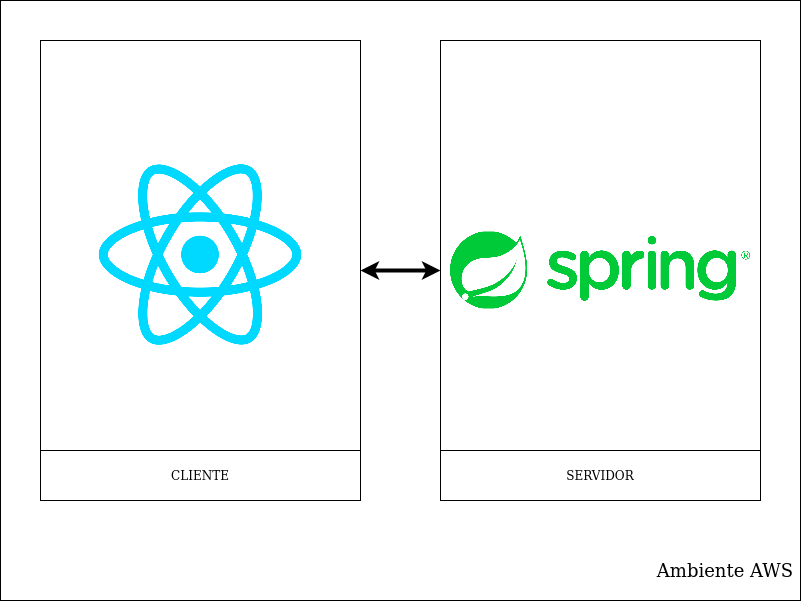
\includegraphics[scale=0.5]{lixt}
  \caption{Arquitetura Lixt}
  \label{fig:cli-srv}
\end{figure}

A comunicação entre estes serviços será feita com o uso do protocolo
\label{sig:http}HTTP, que permite a aplicação cliente realizar chamadas ao servidor
através de urls, seja para buscar informações para apresentar ao
usuário ou postar informações coletadas dele. O framework Spring, além
de abstrair a implementação da lógica de um servidor, implementa
\emph{listeners} para estas urls, auxiliando a criação de pontos na
aplicação do servidor focados na comunicação com a aplicação cliente.

%%% Local Variables:
%%% mode: latex
%%% TeX-master: "../desenho"
%%% End:


% ------------------------------------------------------------------------------
% ------------------------------------------------------------------------------
% Coloquem aqui o include dos capitulos de voces
% e o arquivo correspondente na pasta capitulos
% ------------------------------------------------------------------------------
% ------------------------------------------------------------------------------

\phantompart
\postextual

\bibliography{referencias/referencias}

\end{document}
%%% Local Variables:
%%% mode: latex
%%% TeX-master: t
%%% End:
